\documentclass[12pt, a4]{article}
\usepackage[margin=2cm]{geometry}
\usepackage{parskip}
\usepackage{nameref}
\usepackage{enumitem}
\usepackage{tabularx}
\usepackage{hyperref}
\usepackage[tiny]{titlesec}

\usepackage{amsmath}
\usepackage{amssymb}

\usepackage{fancyhdr}
\usepackage{titling}

\usepackage{pgfplots}
\pgfplotsset{compat=1.16}
\usetikzlibrary{decorations.pathreplacing,positioning, shapes,arrows,chains}


\usepackage{xcolor}
\usepackage{graphicx}
\usepackage{fancyvrb}
\usepackage{listings}
\usepackage{bm}
\usepackage{xcolor}
\usepackage{optidef}


\xdefinecolor{gray}{rgb}{0.4,0.4,0.4}
\xdefinecolor{blue}{RGB}{58,95,205}
\xdefinecolor{darkgreen}{RGB}{0,100,0}

\newcommand{\lightgray}{black!30}

\newcommand{\plotDomain}{-1:8}

\newcommand{\addPlotLDownCoords}[1]{
	\addplot[mark=none, domain=\plotDomain, color=\lightgray,
	decoration={border,segment length=1mm,amplitude=1.5mm,angle=-135},
	postaction={decorate}
	] coordinates {#1};
	\addplot[mark=none, domain=\plotDomain] coordinates {#1};
}

\newcommand{\addPlotLDown}[1]{
	\addplot[mark=none, domain=\plotDomain, color=\lightgray,
	decoration={border,segment length=1mm,amplitude=1.5mm,angle=-135},
	postaction={decorate}
	] {#1};
	\addplot[mark=none, domain=\plotDomain] {#1};
}

\newcommand{\addPlotRUpCoords}[1]{
	\addplot[mark=none, domain=\plotDomain, color=\lightgray,
	decoration={border,segment length=1mm,amplitude=1.5mm,angle=135},
	postaction={decorate}
	] coordinates {#1};
	\addplot[mark=none, domain=\plotDomain] coordinates {#1};
}

\newcommand{\addPlotRUp}[1]{
	\addplot[mark=none, domain=\plotDomain, color=\lightgray,
	decoration={border,segment length=1mm,amplitude=1.5mm,angle=135},
	postaction={decorate}
	] {#1};
	\addplot[mark=none, domain=\plotDomain] {#1};
}

\lstset{% setup listings
	language=R,% set programming language
	basicstyle=\ttfamily\small,% basic font style
	keywordstyle=\color{blue},% keyword style
	commentstyle=\color{gray},% comment style
	numbers=left,% display line numbers on the left side
	numberstyle=\scriptsize,% use small line numbers
	numbersep=10pt,% space between line numbers and code
	tabsize=3,% sizes of tabs
	showstringspaces=false,% do not replace spaces in strings by a certain character
	captionpos=b,% positioning of the caption below
	breaklines=true,% automatic line breaking
	escapeinside={(*}{*)},% escaping to LaTeX
	fancyvrb=true,% verbatim code is typset by listings
	extendedchars=false,% prohibit extended chars (chars of codes 128--255)
	literate={"}{{\texttt{"}}}1{<-}{{$\bm\leftarrow$}}1{<<-}{{$\bm\twoheadleftarrow$}}1
	{~}{{$\bm\sim$}}1{<=}{{$\bm\le$}}1{>=}{{$\bm\ge$}}1{!=}{{$\bm\neq$}}1{^}{{$^{\bm\wedge}$}}1,% item to replace, text, length of chars
	alsoletter={.<-},% becomes a letter
	alsoother={$},% becomes other
	otherkeywords={!=, ~, $, \&, \%/\%, \%*\%, \%\%, <-, <<-, /},% other keywords
	deletekeywords={c}% remove keywords
}



\author{Pascal Lüscher}
\title{Mathematical Optimization – Problem set 5}

\makeatletter
\let\mytitle\@title
\makeatother

\pagestyle{fancy}
\fancyhf{}
\rhead{
	\mytitle\\
	\theauthor
}

\rfoot{
	Page: \thepage
}

\renewcommand{\arraystretch}{1.2} % more space in tables
\renewcommand\thesubsection{\thesection.\alph{subsection}}
\titleformat{\section}[hang]{\normalfont\bfseries\itshape}{\textup{\thesubsection}}{1em}{}

\titleformat{\subsection}[hang]{\normalsize\itshape}{\textup{\thesubsection}}{1em}{}[]

\newcommand{\norm}[1]{\lvert #1 \rvert}

\newcolumntype{L}{>{$}l<{$}} % math-mode version of "l" column type
\newcolumntype{R}{>{$}r<{$}} % math-mode version of "l" column type
\newcolumntype{C}{>{$}c<{$}} % math-mode version of "l" column type


\begin{document}
	\section{Problem 1: Simplex Algorithm}
	Consider the following LP in canonical form:
	
	\begin{tabular}{lCRCRCR}
		max & & x_1 & + & x_2 \\
		s.t. & & x_1 & & &  \leq & 4 \\
		& && & x_2 & \leq & 4 \\
		&&x_1 & + & x_2 & \leq& 7\\
		&-&x_1&-&x_2&\leq&-3\\
		&& x_1 & && \geq &0\\
		&& & &x_2& \geq &0
	\end{tabular}

\subsection{Transform the given linear program into standard form, using slack variables $y1,\ldots,y4$ corresponding to the four constraints (excluding non-negativity constraints).}

\begin{tabular}{lCRCRCRCRCRCRCRR}
	max & & x_1 & + & x_2 \\
	s.t. & & x_1 & & & + & y_1 &&&&&&& = & 4 \\
	& && & x_2 &&&+&y_2&&&& & = & 4 \\
	&&x_1 & + & x_2 &&&&&+&y_3&&& =& 7\\
	&-&x_1&-&x_2&&&&&&&+&y_4&=&-3\\
	&&\multicolumn{11}{L}{x_i,y_j \geq 0 \quad \forall i \in [1,2], \forall j \in [1,2,3,4]}
\end{tabular}

\subsection{Write down the short tableau with basis $B= (y1,y2,y3,y4)$. Is it feasible or infeasible? Why? What is the basic solution in the original space corresponding to this tableau?}
		
	\begin{tabular}{L|RR||R}
		& x_1 & x_2 & 1 \\
		\hline
		z & -1 & -1 & 0 \\
		\hline
		y_1 & 1 & 0 & 4 \\
		y_2 & 0 & 1 & 4 \\
		y_3 & 1 & 1 & 7 \\
		y_4 & -1 & -1 & -3 \\
	\end{tabular}

	This tableau is infeasible since there is a negative $b$ value. The basic solution is $(x_1,x_2,y_1,y_2,y_3,y_4) = (0,0,4,4,7,-3)$ which violates $y_4 \geq 0$
	
\subsection{Run phase I of the Simplex Method to certify feasibility of the problem. From the tableau you obtain, extract a feasible tableau for the given LP.}{\label{sec:1c}}
\begin{minipage}[t]{.3\textwidth}
\begin{tabular}{L|RRR||R}
	& x_1 & x_2 & x_0 & (1) \\
	\hline
	\tilde{z} & 0 & 0 & 1 & 0 \\
	\hline
	z & -1 & -1 & 0 &0 \\
	\hline
	y_1 & 1 & 0 & -1 &4 \\
	y_2 & 0 & 1 & -1 &4 \\
	y_3 & 1 & 1 & -1 &7 \\
	y_4 & -1 & -1 & \fbox{$-1$} & -3 \\
\end{tabular}

most negative row 

\end{minipage}
$\Rightarrow$
\begin{minipage}[t]{.3\textwidth}

	\begin{tabular}{L|RRR||R}
		& x_1 & x_2 & y_4 & (1)  \\
		\hline
		\tilde{z} & -1 & -1 & 1 & -3 \\
		\hline
		z & -1 & -1 & 0 &0 \\
		\hline
		y_1 & 2 & 1 & -1 &7 \\
		y_2 & 1 & 2 & -1 &7 \\
		y_3 & 2 & 2 & -1 &10 \\
		x_0 & \fbox{$1$} & 1 & -1 & 3 \\
	\end{tabular}

row $x_1$ Bland's rule

col $x_0$ quotient rule

\end{minipage}
$\Rightarrow$
\begin{minipage}[t]{.3\textwidth}
	\begin{tabular}{L|RRR||R}
		& x_0 & x_2 & y_4 & (1)  \\
		\hline
		\tilde{z} & 1 & 0 & 0 & 0 \\
		\hline
		z & 1 & 0 & -1    & 3 \\
		\hline
		y_1 & -2 &-1 & 1 & 1 \\
		y_2 & -1 & 1 & 0 & 4 \\
		y_3 & -2 & 0 & 1 & 4 \\
		x_1 & 1  & 1 &-1 & 3 \\
	\end{tabular}

\end{minipage}

$x_0$ equals 0 and optimality is reached so we can delete this column and continue with Simplex phase II to optain the optimal solution for the original LP.

\subsection{Starting from the tableau obtained in \ref{sec:1c}, run phase II of the Simplex Method to obtain an optimal tableau for the given LP, and argue why it is optimal. Read the corresponding solutionand its value from the tableau.}{\label{sec:1d}}

\begin{minipage}[t]{.3\textwidth}
	\centering
	\begin{tabular}{L|RR||R}
		&  x_2 & y_4 & (1)  \\
		\hline
		z &  0 & -1 & 3 \\
		\hline
		y_1 &-1 & \fbox{$1$} & 1 \\
		y_2 & 1 & 0 & 4 \\
		y_3 & 0 & 1 & 4 \\
		x_1 & 1 &-1 & 3 \\
	\end{tabular}
\end{minipage}
$\Rightarrow$
\begin{minipage}[t]{.3\textwidth}
	\centering
	\begin{tabular}{L|RR||R}
		&  x_2 & y_1 & (1)  \\
		\hline
		z &  -1 & 1 & 4 \\
		\hline
		y_4 &-1 & 1 & 1 \\
		y_2 & 1 & 0 & 4 \\
		y_3 & \fbox{1} &-1 & 3 \\
		x_1 & 1 & 1 & 4 \\
	\end{tabular}
\end{minipage}
$\Rightarrow$
\begin{minipage}[t]{.3\textwidth}
	\centering
	\begin{tabular}{L|RR||R}
		&  y_3 & y_1 & (1)  \\
		\hline
		z   & 1 & 0 & 7 \\
		\hline
		y_4 & 1 & 0 & 4 \\
		y_2 &-1 & 1 & 1 \\
		x_2 & 1 &-1 & 3 \\
		x_1 & 0 & 1 & 4 \\
	\end{tabular}
\end{minipage}

This solution is optimal since all coefficients in the objective row ($z$) are non-negative and the tableau is feasible. The optimal solution is $7$ with $(x_1,x_2,y_1,y_2,y_3) = (4,3,0,1,9,4)$.

\pagebreak
\subsection{Draw the feasible region of the initial canonical linear program, mark all solutions that you visited when executing phase I and phase II of the Simplex Method. Use the graphic solution method to double-check that phase II ended at an optimal solution.}{\label{sec:1e}

Simplex-vertices visited in {\color{darkgreen} phase I} and {\color{red} phase II}.
\begin{center}
	\begin{tikzpicture}
		\begin{axis}[
			axis x line=center,
			axis y line=center,
			xlabel=$x_1$,
			ylabel=$x_2$,
			xmin=-1,
			ymin=-1,
			xmax=8,
			ymax=8,
			xtick={0,1,2,...,8},
			ytick={0,1,2,...,8}
			]
			
		
			\addplot[fill=blue!20,draw=none]coordinates{(0,4)(0,3)(3,0)(4,0)(4,3)(3,4)(0,4)};
		

			\addPlotLDown{4} % y_1
			\node[label={20:$y_1$}] at (4,6) {};
			\addPlotLDownCoords{(4,8)(4,-1)} %y_2
			\node[label={10:$y_2$}] at (6,4) {};
			\addPlotLDown{-x + 7}; % y_3
			\node[label={0:$y_3$}] at (6,1) {};
			\addPlotRUp{-x+3}; % y_4
			\node[label={0:$y_4$}] at (1,2) {};
			
			\addPlotRUp{0}; % x_1 >= 0
			\addPlotRUpCoords{(0,8)(0,-1)}; % x_2 >= 0
			
			\addplot[fill=none,draw=blue]coordinates{(0,4)(0,3)(3,0)(4,0)(4,3)(3,4)(0,4)};
		
			\draw[black, ->] (5,5)--(6,6);
			\coordinate[label=c] (c) at (5.5,5.5);
		
			\draw[darkgreen, ->, line width=.75mm] (0,0) -- (3,0);
			\draw[red, ->, line width=.75mm] (3,0) -- (4,0);
			\draw[red, ->, line width=.75mm] (4,0) -- (4,3);

		\end{axis}
	\end{tikzpicture}
\end{center}

Graphical solution
\begin{center}
	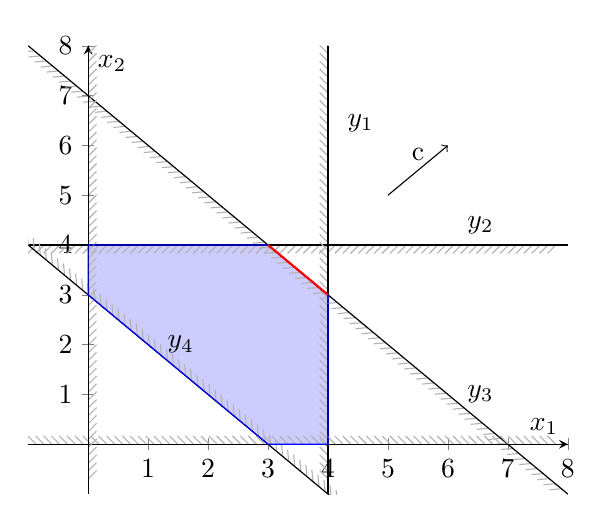
\begin{tikzpicture}
		\begin{axis}[
			axis x line=center,
			axis y line=center,
			xlabel=$x_1$,
			ylabel=$x_2$,
			xmin=-1,
			ymin=-1,
			xmax=8,
			ymax=8,
			xtick={0,1,2,...,8},
			ytick={0,1,2,...,8}
			]
			
			
			\addplot[fill=blue!20,draw=none]coordinates{(0,4)(0,3)(3,0)(4,0)(4,3)(3,4)(0,4)};
			
			
			\addPlotLDown{4} % y_1
			\node[label={20:$y_1$}] at (4,6) {};
			\addPlotLDownCoords{(4,8)(4,-1)} %y_2
			\node[label={10:$y_2$}] at (6,4) {};
			\addPlotLDown{-x + 7}; % y_3
			\node[label={0:$y_3$}] at (6,1) {};
			\addPlotRUp{-x+3}; % y_4
			\node[label={0:$y_4$}] at (1,2) {};
			
			\addPlotRUp{0}; % x_1 >= 0
			\addPlotRUpCoords{(0,8)(0,-1)}; % x_2 >= 0
			
			\addplot[fill=none,draw=blue]coordinates{(0,4)(0,3)(3,0)(4,0)(4,3)(3,4)(0,4)};
			
			\draw[black, ->] (5,5)--(6,6);
			\coordinate[label=c] (c) at (5.5,5.5);
		
			\draw[red, thick] (4,3)--(3,4);
			
		\end{axis}
	\end{tikzpicture}
\end{center}

\subsection{In the drawing from \ref{sec:1e}, you might have observed that there exist infinitely many optimal solutions. Can you argue that this is indeed true by only looking at the optimal tableau obtained in part \ref{sec:1d}?}

Yes, by performing a pivot to bring $y_1$ into basis and $y_2$ out of basis the tableau remains optimal and feasible.

\begin{minipage}[t]{.5\textwidth}
	\centering
	\begin{tabular}{L|RR||R}
		&  y_3 & y_1 & (1)  \\
		\hline
		z   & 1 & 0 & 7 \\
		\hline
		y_4 & 1 & 0 & 4 \\
		y_2 &-1 & \fbox{$1$} & 1 \\
		x_2 & 1 &-1 & 3 \\
		x_1 & 0 & 1 & 4 \\
	\end{tabular}

(Copied from \ref{sec:1d})
\end{minipage}
$\Rightarrow$
\begin{minipage}[t]{.5\textwidth}
	\centering
	\begin{tabular}{L|RR||R}
		&  y_3 & y_2 & (1)  \\
		\hline
		z   & 1 & 0 & 7 \\
		\hline
		y_4 & 1 & 0 & 4 \\
		y_1 &-1 & 1 & 1 \\
		x_2 & 0 & 1 & 4 \\
		x_1 & 1 &-1 & 3 \\
	\end{tabular}
\end{minipage}

\section{Problem 2: Certifying infeasibility from phase I of the Simplex Method }
When solving a linear program of the form
\begin{equation}{\label{eq:1}}
\begin{matrix}
	\text{max}& c^\top x &  & \\ 
	\text{s.t.} & Ax &\leq  &b \\ 
	&  x&\in  & \mathbb{R}^n_{\geq0} 
\end{matrix}
\end{equation}
using the Simplex Method, we start with phase I, where the goal is to decide feasibility of the above linear program, and --- if feasible --- find a feasible vertex solution to start phase II from. To this end, we solve the auxiliary problem
\begin{equation}{\label{eq:2}}
	\begin{matrix*}[r]
		\text{max}& -x_0 &&&  & \\ 
		\text{s.t.} & -1 \cdot x_0 & + & Ax &\leq& b \\ 
		&x_0&&&\in&\mathbb{R}_{\geq0} \\
		&&&x&\in&\mathbb{R}^n_{\geq0} \\
	\end{matrix*}
\end{equation}
and we know that if and only if the optimal value of the latter auxiliary problem is $0$, then the initial linear program is feasible, and we can continue with phase II. The goal of this problem is to show that if the value of the auxiliary problem is strictly negative, then we can obtain a certificate of infeasibility from the corresponding optimal simplex tableau.

\subsection{Show that a vector $\mu \in \mathbb{R}^m_{\geq0}$ with $\mu^\top A\geq0$ and $\mu^\top b <0$ is a certificate of infeasibility of the linear program (\ref{eq:1}). In other words, prove that if such a vector $\mu$ exists, then (\ref{eq:1}) is infeasible.}{\label{sec:2a}}

The vector $\mu$ basicly adds the different constraints together. The linear equation system $Ax \leq b$ and $\mu^\top A \leq \mu^\top b$ is equal. For simplicity I define $A' = \mu^\top A$ and $b' = \mu^\top b$. If $A' \geq 0$ and $b' < 0$ there is no $x \in \mathbb{R}^n_{\geq 0}$ such that $A'x \leq b'$ becuase $x$ is larger equal than zero (positive) and so is $A'$. but $b'$ is strictly negative.

\subsection{Consider the case where the auxiliary problem (\ref{eq:2}) has a strictly negative optimal value. What can you say about an optimal short tableau of the corresponding standard form problem?}{\label{sec:2b}}

\subsection{Use properties of the optimal tableau considered in \ref{sec:2b} to find a certificate vector $\mu \in \mathbb{R}^m_{\geq0}$ as discussed in \ref{sec:2a}}

\pagebreak
\section{Problem 3: The dual of a general linear program}
In class, the dual problem of an linear program in canonical form was defined. The goal of this exercise is to derive the dual of a linear program given in the following most general form

\begin{equation}{\label{eq:p}}
	\begin{matrix*}[r]
		\text{max} & d^\top x & + & e^\top y & + & f^\top z \\
		\text{s.t.} & Ax & + & By & + & Cz & \leq & a \\	
		            & Dx & + & Ey & + & Fz & = & b \\	
		            & Gx & + & Hy & + & Kz & \geq & c		      \\	      
		            &    &   &    &   & x  & \in & \mathbb{R}^{n_d}_{\geq 0} \\
		            &    &   &    &   & y  & \in & \mathbb{R}^{n_e}\\
		            &    &   &    &   & z  & \in & \mathbb{R}^{n_f}_{\leq 0}\\		            		            
	\end{matrix*}
\end{equation}

\subsection{Transform the linear program (\ref{eq:p}) into an linear program in canonical form and write down the corresponding dual program.}{\label{sec:3a}}

To transform the LP into canonical the $\geq$--constraints will be multiplied with $-1$. The $=$--constraints will be replaced by a $\leq$ and $\geq$ constraint. The $\geq$--constraint will then be multiplied with $-1$ to create a $\leq$-- constraint.
To bring all variables in $\mathbb{R}_{\geq 0}$, the variable $y$ gets replaced by $y_1 - y_2$ and $z$ is multiplied by $-1$

\begin{equation}{\label{eq:p_canonical}}
	\begin{matrix*}[r]
		\text{max} & d^\top x & + & e^\top (y_1-y_2) & - & f^\top z \\
		\text{s.t.} & Ax & + & B(y_1-y_2) & - & Cz & \leq & a \\	
		& Dx & + & E(y_1-y_2) & - & Fz & \leq & b \\	
		& -Dx & - & E(y_1-y_2) & + & Fz & \leq & -b \\	
		& -Gx & - & H(y_1-y_2) & + & Kz & \leq & -c		      \\	      
		&    &   &    &   & x  & \in & \mathbb{R}^{n_d}_{\geq 0} \\
		&    &   &    &   & y_1, y_2  & \in & \mathbb{R}^{n_e}_{\geq 0}\\
		&    &   &    &   & z  & \in & \mathbb{R}^{n_f}_{\geq 0}\\		            		            
	\end{matrix*}
\end{equation}


The dual problem according to the rules is the following. (i choose $\delta$ for the slack variables)

\begin{equation}{\label{eq:p_dual}}
	\begin{matrix*}[r]
		\text{min} &a^\top \delta_1 & + & b^\top \delta_2 &- & b^\top \delta_3 & - & c^\top \delta_4   \\
\text{s.t.} & A^\top \delta_1  & + & D^\top \delta_2 & - & D^\top \delta_3 & - & G^\top \delta_4&\geq & d \\
            & B^\top \delta_1  & + & E^\top \delta_2 & - & E^\top \delta_3 & - & H^\top \delta_4 &\geq & e \\	
  			& -B^\top \delta_1 & - & E^\top \delta_2 & + & E^\top \delta_3 & + & H^\top \delta_4 &\geq & -e \\	
	  		& -C^\top \delta_1 & - & F^\top \delta_2 & + & F^\top \delta_3 & + & K^\top \delta_4 &\geq & -f \\	

		&    &   &    &   &&& \delta_1  & \in & \mathbb{R}^{m_a}_{\geq0} \\
		&    &   &    &   &&& \delta_2, \delta_3  & \in & \mathbb{R}^{m_b}_{\geq0} \\
		&    &   &    &   &&& \delta_4  & \in & \mathbb{R}^{m_c}_{\geq0} \\						
	\end{matrix*}
\end{equation}

\subsection{We say that two linear programs are equivalent if every feasible solution of one of the problems can be transformed into a feasible solution of the other problem with the same objective value. Prove that the dual linear program from \ref{sec:3a} is equivalent to the following linear program (\ref{eq:d})}{\label{sec:3b}}
\begin{equation}{\label{eq:d}}
	\begin{matrix*}[r]
		\text{min} & a^\top u &+& b^\top v &+& c^\top w && \\
		\text{s.t.} & A^\top u &+& D^\top v &+& G^\top w & \geq & d \\
					& B^\top u &+& E^\top v &+& H^\top w & = & e \\
					& C^\top u &+& F^\top v &+& K^\top w & \leq & f \\		
					&&&&&u&\in&\mathbb{R}^{m_a}_{\geq 0} \\	
					&&&&&v&\in&\mathbb{R}^{m_b} \\	
					&&&&&w&\in&\mathbb{R}^{m_c}_{\leq 0} \\
	\end{matrix*}
\end{equation}

First step: Create the $=e$ constraint by combining row $2$ and $3$:

\begin{equation}{\label{eq:p_dual_eqe}}
	\begin{matrix*}[r]
		\text{min} &a^\top \delta_1 & + & b^\top \delta_2 &- & b^\top \delta_3 & - & c^\top \delta_4   \\
		\text{s.t.} & A^\top \delta_1  & + & D^\top \delta_2 & - & D^\top \delta_3 & - & G^\top \delta_4&\geq & d \\
		& B^\top \delta_1  & + & E^\top \delta_2 & - & E^\top \delta_3 & - & H^\top \delta_4 & = & e \\	
		& -C^\top \delta_1 & - & F^\top \delta_2 & + & F^\top \delta_3 & + & K^\top \delta_4 &\geq & -f \\	
		
		&    &   &    &   &&& \delta_1  & \in & \mathbb{R}^{m_a}_{\geq0} \\
		&    &   &    &   &&& \delta_2, \delta_3  & \in & \mathbb{R}^{m_b}_{\geq0} \\
		&    &   &    &   &&& \delta_4  & \in & \mathbb{R}^{m_c}_{\geq0} \\									
	\end{matrix*}
\end{equation}

Then we create the $\leq$--constraint for $f$ by multiplying the row by $-1$

\begin{equation}{\label{eq:p_dual_leqf}}
	\begin{matrix*}[r]
		\text{min} &a^\top \delta_1 & + & b^\top \delta_2 &- & b^\top \delta_3 & - & c^\top \delta_4   \\
		\text{s.t.} & A^\top \delta_1  & + & D^\top \delta_2 & - & D^\top \delta_3 & - & G^\top \delta_4&\geq & d \\
		& B^\top \delta_1  & + & E^\top \delta_2 & - & E^\top \delta_3 & - & H^\top \delta_4 & = & e \\	
		& C^\top \delta_1 & + & F^\top \delta_2 & - & F^\top \delta_3 & - & K^\top \delta_4 &\leq & f \\	
		
		&    &   &    &   &&& \delta_1  & \in & \mathbb{R}^{m_a}_{\geq0} \\
		&    &   &    &   &&& \delta_2, \delta_3  & \in & \mathbb{R}^{m_b}_{\geq0} \\
		&    &   &    &   &&& \delta_4  & \in & \mathbb{R}^{m_c}_{\geq0} \\									
	\end{matrix*}
\end{equation}

Replace $\delta_2 - \delta_3$ by $v$. Since both are positive, $v$ is in $\mathbb{R}^{n_b}$

\begin{equation}{\label{eq:p_dual_v}}
	\begin{matrix*}[r]
		\text{min} &a^\top \delta_1 & + & b^\top v & - & c^\top \delta_4   \\
		\text{s.t.} & A^\top \delta_1  & + & D^\top v & - & G^\top \delta_4&\geq & d \\
		& B^\top \delta_1  & + & E^\top v & - & H^\top \delta_4 & = & e \\	
		& C^\top \delta_1 & + & F^\top v & - & K^\top \delta_4 &\leq & f \\	
		
		&    &   &    &   &&& \delta_1  & \in & \mathbb{R}^{m_a}_{\geq0} \\
		&    &   &    &   &&& v  & \in & \mathbb{R}^{m_b} \\
		&    &   &    &   &&& \delta_4  & \in & \mathbb{R}^{m_c}_{\geq0} \\									
	\end{matrix*}
\end{equation}


To bring $\delta_4$ in $\mathbb{R}^{n_c}_{\leq 0}$ I multiply it by $-1$ and rename it to $w$.

\begin{equation}{\label{eq:p_dual_w}}
	\begin{matrix*}[r]
		\text{min} &a^\top \delta_1 & + & b^\top v & + & c^\top w   \\
		\text{s.t.} & A^\top \delta_1  & + & D^\top v & + & G^\top w&\geq & d \\
		& B^\top \delta_1  & + & E^\top v & + & H^\top w & = & e \\	
		& C^\top \delta_1 & + & F^\top v & + & K^\top w &\leq & f \\	
		
		&    &   &    &   &&& \delta_1  & \in & \mathbb{R}^{m_a}_{\geq0} \\
		&    &   &    &   &&& v  & \in & \mathbb{R}^{m_b} \\
		&    &   &    &   &&& w  & \in & \mathbb{R}^{m_c}_{\leq0} \\									
	\end{matrix*}
\end{equation}
Rename $\delta_1$ to $u$

\begin{equation}{\label{eq:p_dual_u}}
	\begin{matrix*}[r]
		\text{min} &a^\top u & + & b^\top v & + & c^\top w   \\
		\text{s.t.} & A^\top u  & + & D^\top v & + & G^\top w&\geq & d \\
		& B^\top u  & + & E^\top v & + & H^\top w & = & e \\	
		& C^\top u & + & F^\top v & + & K^\top w &\leq & f \\	
		
		&    &   &    &   &&& u  & \in & \mathbb{R}^{m_a}_{\geq0} \\
		&    &   &    &   &&& v  & \in & \mathbb{R}^{m_b} \\
		&    &   &    &   &&& w  & \in & \mathbb{R}^{m_c}_{\leq0} \\									
	\end{matrix*}
\end{equation}

\pagebreak
\section{Problem 4: Primal and dual pivot}

Consider the following linear program in canonical form.
\begin{equation}{\label{eq:p_1}}
	\begin{matrix}
		\text{max}& c^\top x &  & \\ 
		\text{s.t.} & Ax &\leq  &b \\ 
		&  x&\in  & \mathbb{R}^n_{\geq0} 
	\end{matrix}
\end{equation}
In class, it was shown that performing an exchange step on a non-zero pivot in the tableau corresponding to (\ref{eq:p_1}) leads to a new tableau corresponding to a linear program equivalent to (\ref{eq:p_1}). In this problem, we show that the two dual problems corresponding to the primal tableaus before and after the pivot step are equivalent, as well. In other words, we show that the following diagram commutes:
\begin{center}
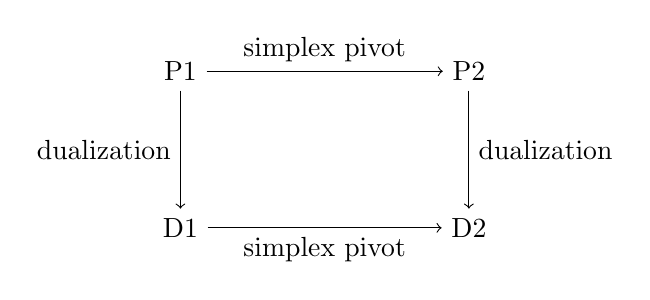
\begin{tikzpicture}
	\node (P1) {P1};
	\node[right=3cm of P1] (P2) {P2};
	\node[below=1.5cm of P1] (D1) {D1};
	\node[below=1.5cm of P2] (D2) {D2};
	
	\draw[->] (P1) -- node [midway,above]  {simplex pivot} (P2);
	\draw[->] (D1) -- node [midway,below]  {simplex pivot} (D2);
	
	\draw[->] (P1) -- node [midway,left]  {dualization} (D1);
	\draw[->] (P2) -- node [midway,right]  {dualization} (D2);
	
\end{tikzpicture}
\end{center}
Recall that we have seen in the lecture that pivoting steps in simplex tableaus transform the underlying primal system into an equivalent system of equations. Commutativity of the above diagram implies that this is also true for the systems that we get from the dual reading of the tableaus. In the following, assume that the entry $A_{ij}$ in the $i^{\text{th}}$ row and $j^{\text{th}}$ column of $A$ is non-zero.

\subsection{Write down the short tableau corresponding to (\ref{eq:p_1}) and perform a pivot step on $A_{ij}$. Write down the new tableau, i.e., calculate its entries in terms of the entries of the old tableau.}{\label{sec:4a}}

\begin{equation}
	\begin{array}{c|ccccc|c}
		& x_1 & \ldots & x_j & \ldots & x_n & 1 \\
		\hline
		z & -c_1 & \ldots & -c_j & \ldots & -c_n & 0 \\
		\hline
		y_1 & A_{11} & \ldots & A_{1j} & \ldots & A_{1n} & b_j \\
		\vdots & \vdots && \vdots & & \vdots & \vdots \\
		y_i & A_{i1} & \ldots & \fbox{$A_{ij}$} & \ldots & A_{in} & b_i \\
		\vdots & \vdots && \vdots & & \vdots & \vdots \\
		y_m & A_{m1} & \ldots & A_{mj} & \ldots & A_{mn} & b_m \\
	\end{array}
	\label{eq:p_1_short_tableau}
\end{equation}


\begin{equation}
	\Rightarrow
	\begin{array}{c|ccccc||c}
		& x_1 & \ldots & y_i & \ldots & x_n & 1 \\
		\hline
		z & -c_1-\frac{c_jA_{i1}}{A_{ij}} & \ldots & \frac{c_j}{A_{ij}} & \ldots & -c_n-\frac{c_jA_{in}}{A_{ij}} & -\frac{c_jb_i}{A_{ij}} \\
		\hline
		y_1 & A_{11}-\frac{A_{1j}A_{i1}}{A_{ij}} & \ldots & -\frac{A_{1j}}{A_{ij}} & \ldots & A_{1n}-\frac{A_{1j}A_{in}}{A_{ij}} & b_1-\frac{A_{1j}b_{i}}{A_{ij}} \\
		\vdots & \vdots && \vdots & & \vdots & \vdots \\
		x_j & \frac{A_{i1}}{A_{ij}} & \ldots & \frac{1}{A_{ij}} & \ldots & \frac{A_{in}}{A_{ij}} & \frac{b_i}{A_{ij}} \\
		\vdots & \vdots && \vdots & & \vdots & \vdots \\
		y_m & A_{m1}-\frac{A_{mj}A_{i1}}{A_{ij}} & \ldots & -\frac{A_{mj}}{A_{ij}} & \ldots & A_{mn}-\frac{A_{mj}A_{in}}{A_{ij}} & b_m - \frac{A_{mj}b_{i}}{A_{ij}} \\
	\end{array}
	\label{eq:p_1_short_tableau_pivoted}
\end{equation}

\subsection{Formulate the dual of the problem that corresponds to the tableau you got in (\ref{sec:4a}), transform it to canonical form, and write down the short tableau for this problem.}{\label{sec:4b}}

Dual problem of \ref{eq:p_1_short_tableau_pivoted}

\begin{equation}
	\begin{array}{c|ccccc||c}
		& y_1 & \ldots & x_j & \ldots & y_m & 1 \\
		\hline
		z & b_1-\frac{A_{1j}b_{i}}{A_{ij}} & \ldots & \frac{b_i}{A_{ij}} & \ldots & b_m - \frac{A_{mj}b_{i}}{A_{ij}} & -\frac{c_jb_i}{A_{ij}} \\
		\hline
		x_1 & A_{11}-\frac{A_{1j}A_{i1}}{A_{ij}} & \ldots & \frac{A_{i1}}{A_{ij}} & \ldots & A_{m1}-\frac{A_{mj}A_{i1}}{A_{ij}} & -c_1-\frac{c_jA_{i1}}{A_{ij}} \\
		\vdots & \vdots && \vdots & & \vdots & \vdots \\
		y_i & -\frac{A_{1j}}{A_{ij}} & \ldots & \frac{1}{A_{ij}} & \ldots & -\frac{A_{mj}}{A_{ij}} & \frac{c_j}{A_{ij}} \\
		\vdots & \vdots && \vdots & & \vdots & \vdots \\
		x_n & A_{1n}-\frac{A_{1j}A_{in}}{A_{ij}}  & \ldots & \frac{A_{in}}{A_{ij}} & \ldots & A_{mn}-\frac{A_{mj}A_{in}}{A_{ij}} & -c_n-\frac{c_jA_{in}}{A_{ij}} \\
	\end{array}
	\label{eq:p_1_dual_short_tableau_pivoted}
\end{equation}

Canonical form of the pivoted dual problem (\ref{eq:p_1_dual_short_tableau_pivoted}):

{\color{red} INSERT CANONICAL FORM HERE}

\subsection{Now first dualize (\ref{eq:p_1}), transform it to canonical form, and write down the short tableau for this problem.}{\label{sec:4c}}

Dual problem of \ref{eq:p_1}:
\begin{equation}{\label{eq:p_1_dual}}
	\begin{matrix}
		\text{min}& b^\top y &  & \\ 
		\text{s.t.} & A^\top y &\geq  &c\\ 
		&  y&\in  & \mathbb{R}^m_{\geq0} 
	\end{matrix}
\end{equation}

canonical form
\begin{equation}{\label{eq:p_1_dual_canonical}}
	\begin{matrix}
		-\text{max}& -b^\top y &  & \\ 
		\text{s.t.} & -A^\top y &\leq  &-c\\ 
		&  y&\in  & \mathbb{R}^m_{\geq0} 
	\end{matrix}
\end{equation}

tableau
\begin{equation}{\label{eq:p_1_dual_tableau}}
	\begin{array}{c|ccccc|c}
		& y_1 & \ldots & y_i & \ldots & y_m & 1 \\
		\hline
		z & b_1 & \ldots & b_j & \ldots & b_m & 0 \\
		\hline
		x_1 & -A_{11} & \ldots & -A_{i1} & \ldots & -A_{m1} & -c_1 \\
		\vdots & \vdots && \vdots & & \vdots & \vdots \\
		x_j & -A_{1j} & \ldots & -A_{ij} & \ldots & -A_{mj} & c_j \\
		\vdots & \vdots && \vdots & & \vdots & \vdots \\
		x_n & -A_{1n} & \ldots & -A_{in} & \ldots & -A_{mn} & c_n \\
	\end{array}
\end{equation}

\subsection{In the tableau obtained in (\ref{sec:4c}), perform a pivot step on the entry in the $j^\text{th}$ row and $i^\text{th}$ column. Write down the new tableau, i.e., calculate its entries in terms of the entries of the old tableau.}{\label{sec:4d}}

\begin{equation}
	\begin{array}{c|ccccc||c}
		& y_1 & \ldots & x_j & \ldots & y_m & 1 \\
		\hline
		z & b_1-\frac{A_{1j}b_{i}}{A_{ij}} & \ldots & \frac{b_i}{A_{ij}} & \ldots & b_m - \frac{A_{mj}b_{i}}{A_{ij}} & -\frac{c_jb_i}{A_{ij}} \\
		\hline
		x_1 & A_{11}-\frac{A_{1j}A_{i1}}{A_{ij}} & \ldots & \frac{A_{i1}}{A_{ij}} & \ldots & A_{m1}-\frac{A_{mj}A_{i1}}{A_{ij}} & -c_1-\frac{c_jA_{i1}}{A_{ij}} \\
		\vdots & \vdots && \vdots & & \vdots & \vdots \\
		y_i & -\frac{A_{1j}}{A_{ij}} & \ldots & \frac{1}{A_{ij}} & \ldots & -\frac{A_{mj}}{A_{ij}} & \frac{c_j}{A_{ij}} \\
		\vdots & \vdots && \vdots & & \vdots & \vdots \\
		x_n & A_{1n}-\frac{A_{1j}A_{in}}{A_{ij}}  & \ldots & \frac{A_{in}}{A_{ij}} & \ldots & A_{mn}-\frac{A_{mj}A_{in}}{A_{ij}} & -c_n-\frac{c_jA_{in}}{A_{ij}} \\
	\end{array}
	\label{eq:p_1_dual_short_tableau_pivoted}
\end{equation}

\subsection{Observe that in (\ref{sec:4b}) and (\ref{sec:4d}), you obtained the same tableaus, and conclude that indeed, the diagram given above commutes.}
It does $:)$


\end{document}

